\section{Architecture Patterns or Styles}
	\subsection{Layered Architectural Strategy}
	The OnlyRugby application will make use of a 4-tier layered pattern, as explained below:
	\begin{enumerate}
		\item Presentation Layer:
		The Presentation Layer is comprised of two main aspects:
		\begin{enumerate}
			\item Interface: Provides an interface/front-end through which users/clients can access and interact with the Application Layer.
			\item Client Data Access: Captures the client's input and and passes it on to the Application Layer. Also responsible for validating input (but not for authentication).
		\end {itemize}
		\item Application Layer:
		\begin{itemize}
			\item Provides back-end services of the system (i.e. all functions and forms of data processing/manipulation).
			\item Manages access to the web-services layer.
			\item Manages client login authentication.
			\item Manages persistence to the main database.
			\item If the app can not currently reach the database then this layer will provide a space to temporarily store all relevant data which needs to be uploaded to the database at a later time.
		\end {itemize}
		\item Web-services Layer:
		This layer is where the server is situated.
		\begin{itemize}
			\item Receives the processed client input from the Application Layer and adds it to the database (i.e. allows reading from- and writing to database).
			\item Provides other server-side computation/services such as:
				\begin{itemize}
					\item Conflict resolution when two different clients upload match statistics.
					\item Sending emails to clients (for example when registering with OnlyRugby).
				\end{itemize}
		\end{itemize}
		\item Data Layer:
		This layer is where the database is situated.
		\begin{itemize}
			\item Stores all added information, even when the client is not communicating with the database (i.e. persists data).
		\end{itemize}

		Reasons for choosing a layered architecture:
		\begin{itemize}
			\item Complexity is reduced by abstracting and separating a number of well defined layers which are then weakly coupled with each other. This allows the responsibilities of the system to be divided between the different layers and can prevent certain aspects of the system from becoming too dependant on (or needlessly intertwined with) another aspect of the system.
			\item It allows for the possibility of layers, at times, being re-used across the system (for example the Presentation Layer relies on the Application Layer to verify all input whereas the Web-services Layer relies on the Application Layer to format the input so that it could be stored in the database).
			\item Separating certain aspects (such as interface and implementation) makes it easier to separate test different parts of the system.
			\item The reduced dependency of various parts of the system on each other will also improve maintainability as it allows parts of the system to be updated without requiring any unnecessary changes to other parts of the system.
		\end{itemize}
		\begin{center}
  	 		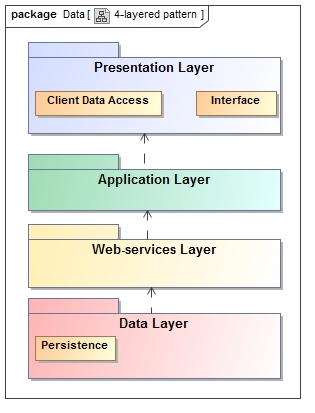
\includegraphics[width=1\textwidth] {4-layered pattern.jpg}\\[0.4cm]    
		\end{center}
	\end{enumerate}